\documentclass[12pt, a4paper, oneside]{ctexbook}
\usepackage{amsmath, amsthm, amssymb, bm, graphicx, hyperref, mathrsfs,diagbox
 ,multicol, tipa,pdfpages}

\title{{\Huge{\textbf{NOTE}}}\\}
\author{理塘顶真·cxk}
\date{\today}
\linespread{1.5}
\newtheorem{theorem}{定理}[section]
\newtheorem{definition}[theorem]{定义}
\newtheorem{lemma}[theorem]{引理}
\newtheorem{corollary}[theorem]{推论}
\newtheorem{example}[theorem]{例}
\newtheorem{proposition}[theorem]{命题}


\begin{document}

\maketitle

\pagenumbering{roman}
\setcounter{page}{1}

\begin{center}
    \Huge\textbf{前言}
\end{center}~\

这是笔记的前言部分. 
~\\
\begin{flushright}
    \begin{tabular}{c}
        Dylaaan\\
        \today
    \end{tabular}
\end{flushright}

\newpage
\pagenumbering{Roman}
\setcounter{page}{1}
\tableofcontents
\newpage
\setcounter{page}{1}
\pagenumbering{arabic}

\chapter{writing}
\section{Class 4}
Directions: For this part, you are allowed 30 minutes to write an essay that begins with the sentence 
“Nowadays parents are increasingly aware that allowing kids more freedom to explore and learn on their own helps foster their independence and boost their confidence.” 
You can make comments, cite examples or use your personal experiences to develop your essay. 
You should write at least 150 words but no more than 200 words not including the sentence given.
~\\


主体:父母,家庭教育
~\\


家长给自由:角色:
~\\


Nowadays parents are increasingly aware that allowing kids more freedom to explore and learn on their own 
helps foster their independence and boost their confidence. 


The understanding, however, leads to a widely debated topic: to what extent should children be given freedom. 
While the question cannot be answered with precise numbers, it highlights the need to define the role of parents in their children’s journey of exploration and learning.(把抽象的变具体)


True freedom for children involves providing opportunities for exploration within a framework of guidance and safety, rather than unchecked liberty.
(放肆的自由). (上一句笼统概括、下定义,下一句写具体的例子,要注意把每一个抽象的要素转化为具体的东西)
People should create an environment where children can pursue their interests, make decisions and… 
with the understanding that boundaries and support are readily available when needed.


The role of the parent is thus not diminished but transformed into that of a mentor who guides, advises and supports.
(下定义:…不是…,而是超越了…)父母不应该只教孩子使用电子产品,而更应该教如何培养数字时代的素养、批判性思维等


In conclusion, providing children with the freedom to explore and … is a adj. art that requires parents to …(后面补充要注意的点) 
It’s about creating a secure foundation on which children can build as they stretch their wings. In the words of Maria Montessori, 
“The greatest gifts we can give our children are the roots of responsibility and the wings of independence.” (纠正青少年观念)


蒙氏教育
\section{Class 5}
Directions: For this part, you are allowed 30 minutes to write an essay that begins with the sentence "Today more and more people begin to realize the pleasures and joys of real-world social interaction." 
You can make comments, cite examples or use your personal experiences to develop your essay. You should write at least 150 words but no more than 200 words. 
~\\


Today more and more people begin to realize the pleasures and joys of real-world social interaction. 
(通过问题引起下文) In an age where technological 
advancements promise to shrink the world and 
bring us closer, \textbf{a paradoxical scenario}(插入比喻) 
unfolds: (具体讲什么变远,什么变近)(\textbf{具体})the more 
connected we are by technology, the wider the 
emotional and psychological gaps between us 
seem to grow. This contradiction hints at 
(hint v. 暗示  hint at sth)
a truth: 现实更重要


(拿网恋做反例)


The reason is simple: the emotional impact of 
physically being with someone and the unspoken 
understanding(心照不宣的默契) that comes from a 
glance or a touch cannot be replicated
(replicate v. 复制\quad 无法被替代:cannot be replicated)
 by digital means. (人际交往都可以用)Many relationships start 
 with texts and virtual chats, where emotions 
 and sentiments are exchanged through screens. 
 Yet, no matter how intense these digital 
 exchanges might be, they \textbf{pale}(v. 苍白、逊色) 
 in comparison to the moment when two people 
 hold hands for the first time.(\textbf{when
..., everything else pales in comparison}) 
Similarly, during disagreements that inevitably 
arise in any relationship, a single real-life 
hug can \textbf{melt} away misunderstanding, 
which is feat that countless online apologies 
might fail to achieve.


(先批驳,然后揭露本质)Realizing the pleasures 
and joys of real-world social interaction 
teaches us a lesson(网恋这个例子只是工具) about 
human nature. (转换的同时对上文总结)It 
underscores(v. 突出) our need for genuine 
connections that go beyond digital communications. 
These interactions, with all the imperfections, 
allow us to feel deeply, understand profoundly 
and connect on a level that digital platforms 
can never fully accomodate.


The words of \textbf{Maya Angelou} resonate(v. 产生共鸣) 
deeply: \textbf{ ``People will forget what you said, 
people will forget what you did, but people 
will never forget how you made them 
feel." }(表白金句) It's the pleasures and joys 
of real-world social interaction that truly 
affirms our existence of empathy, connection 
and love.
\section{Class 6}
Directions: For this part, you are allowed 30 minutes to write an essay that begins with the 
sentence ``Nowadays more and more people take delight in offering help to the needy." You 
can make comments, cite examples, or use your personal experiences to develop your essay. 
You should write at least 150 words but no more than 200 words.
~\\


给出观点$\Rightarrow$引出一个相关现象,把抽象的观点具象化
$\Rightarrow$举例$\Rightarrow$给出正确的定义$\Rightarrow$总结
~\\


Nowadays more and more people take delight in offering help to the needy. 
(不废话的肯定)In a world marred(v. 破坏,糟蹋) 
by individualism and materialism, seeing people 
extend a helping hand to those in less fortunate 
circumstances is indeed \textbf{
    a scene  that we all yearn(v. 渴望) to witness. (...是我们渴望看到的,引出话题)
}
However, assisting others is not without its challenges and costs. 
Everyone has their own concerns and limitations, 
and our efforts should be to encourage and support 
rather judge or criticize.
~\\


界定道德绑架这个概念:通过质疑别人的道德,强迫别人做...
~\\

(解释概念$\Rightarrow$举例,这样做的不好之处)


Now, the phenomenon of ``moral hijacking(hijack v. 绑架)" has become 
increasingly prevalent. This concept refers to 
the practice of compelling individuals or 
organizations to support a cause by questioning 
their morality or ethics, often leveraging(v. 利用) 
social media as a platform for exerting pressure. 
During fundraising(fundraise v. 募捐) certain campaigns, people 
might feel coerced(coerce v. 强制,威胁) into donating 
because failure to do so could result in being 
labeled as indifferent or selfish by the community. 
Such tactics not only create an atmosphere of guilt 
and obligation but can also lead to resentment 
and a decrease in genuine acts of charity. 


In fact, offering help, whether it be(后面既有单数又有复数可以直接用be) through 
volunteering, financial donations, or simply 
lending an ear, often demands time, energy 
and resources. For some, these are readily 
available, but for others, there may be significant 
personal or financial constraints that make 
such contributions difficult. It's important 
to recognize that every little act of kindness 
counts, regardless of its scale.


\textbf{Not all of us can do great things. But we can do 
small things with great love.(用心做事、哪怕渺小也能做大事)} 
By valuing each act of kindness, irrespective 
of size(irrespective adj. 不考虑 irrespective of sth 不考虑...), we cultivate a more compassionate and 
understanding society, one that cherishes 
the spirit of giving while respecting individual 
boundaries and capacities.

\chapter{六级真题}
\section{2022.6第一套}
\begin{multicols}{2}
    \begin{itemize}
        \item [1.]staff writer 职业撰稿人
        \item [2.]eidtorial adj. 编辑的
        \item [3.]proofread v. 校对(与read相似,
        proofread-proofread)
        \item [4.]graphic novel 漫画书
        \item [5.]demographically adv. 人口统计地
        \item [6.]put aside 存钱
        \item [7.]thriftiness n. 节俭
        \item [8.]thrifty adj. 节俭的
        \item [9.]means n. 财富,金钱
        

        beyond the means of most people\quad 是大多数人无力消费的
        \item [10.]fall short 没达到预期
        \item [11.]count on 依靠,指望
        \item [11.]see your plans through 完成你的计划
        \item [12.]lifestyle creep 生活方式的改变
    \end{itemize}
\end{multicols}
\section{2022.9第一套}
\begin{multicols}{2}
    \begin{itemize}
        \item [1.]adhere v. 黏附(=stick)
        

        (adhered-adhered)


        adhere to sth 坚持,遵守
        \item [2.]tumble v.\&n. 摔倒、翻滚
        

        tumble dryer 滚筒式烘干机
        \item [3.]overlook v. 俯视,忽略
        \item [4.]glamorous adj. 吸引人的
        \item [5.]deposit n. 订金,押金,存款
        \item [6.]mandatory adj. 必须的,法律要求的
        \item [7.]tenant n. 房客,租户
        \item [8.]baffle v. 使困惑
        
        e.g.His behavior baffles me.
        \item [9.]detrimental adj. 有害的
        \item [10.]incentive n. 激励,鼓励
        
        tax incentives to encourage savings\quad 鼓励储蓄的税收措施
        \item [11.]suppress v. 抑制,镇压,禁止
        \item [12.]ethic n. 道德
        \item [13.]infer v. 推断,暗示
        \item [14.]hypocrisy n. /\textipa{hI'pA:kr@si}/
        
        伪善,虚伪
        \item [15.]hypocritical adj. 虚伪的,伪善的
        \item [16.]tactic n. 方法、战术
        \item [17.]outright adj.\&adv. 完全彻底的;公开直接的
        \item [18.]concede v. 承认
        \item [19.]notwithstanding prep.\&adv. 尽管
        \item [20.]scrutiny n. 仔细审查
        \item [21.]scrutinize v. 仔细审查
        \item [22.]recollection n. 记忆,回忆
        \item [23.]complementary adj. 互补的
        \item [24.]speak of 谈及
        \item [25.]responsive adj. 反应积极的;热情的
        
        be responsive to 对...做出积极反应;对...热情
        \item [26.]susceptible adj. 易受...影响(或伤害);多愁善感的
        
        be susceptible to... 容易受...影响
        

        be susceptible of... 可以...的


        e.g.1:He's highly susceptible to flattery.他爱听恭维话


        e.g.2:She was both charming and susceptible.她迷人而多情


        e.g.3:Is this situation not susceptible of improvement by legislation?
        这种状况不能通过立法加以改善吗?
        \item [27.]alliance n. 联盟、同盟
        

        alliance between A and B
        \item [28.]undercurrent n. 潜在的情绪(尤指负面)
        \item [29.]permeate v. (气体、液体)渗透、弥漫;(思想、影响)感染、传播
        \item [30.]dissimilar adj. 不同的
        \item [31.]apt adj. 恰当的;有...倾向的
        

        be apt to do 容易...
        \item [32.]precedence n. 优先;优先权
        

        take (sharper) precedence over 比...更重要


        in order of precedence 按照重要次序排列


        e.g.Dating and relationships with boys take sharper precedence over sisterhood.
        和男生的关系比姐妹关系更重要
        \item [33.]dilute v. 冲淡、稀释、削弱
        \item [34.]dubious adj. 怀疑,可疑的,不一定的
        
        be dubious about... 对...怀疑
        \item [35.]indigenous adj. 本地的
        
        (=native)
        \item [36.]specimen n. 样品,样本
        \item [37.]refuge n. 庇护;避难所
        
        take/seek refuge from... 寻求庇护躲\dots
        \item [38.]expire v. 到期;去世
        
        sth expire ... 到期/去世
        \item [39.]deplete v. 大量减少(usually passive)
        
        Food supplies were severely depleted.食物供应已严重不足
        \item [40.]legislature n. 立法机构
        \item [41.]bill n. 议案、法案
        \item [42.]monolingual adj. 只使用一种语言的
        
        bilingual adj. 会两种语言的
        \item [43.]immersive adj. 沉浸式的、身临其境的
        \item [44.]ethnicity n. the state or fact of 
        belonging to a particular ethic group
        \item [45.]lag v. 落后
        
        lag behind... 落后于\dots
    \end{itemize}
\end{multicols}

\chapter{外刊}
\section{2024.4.11外刊}
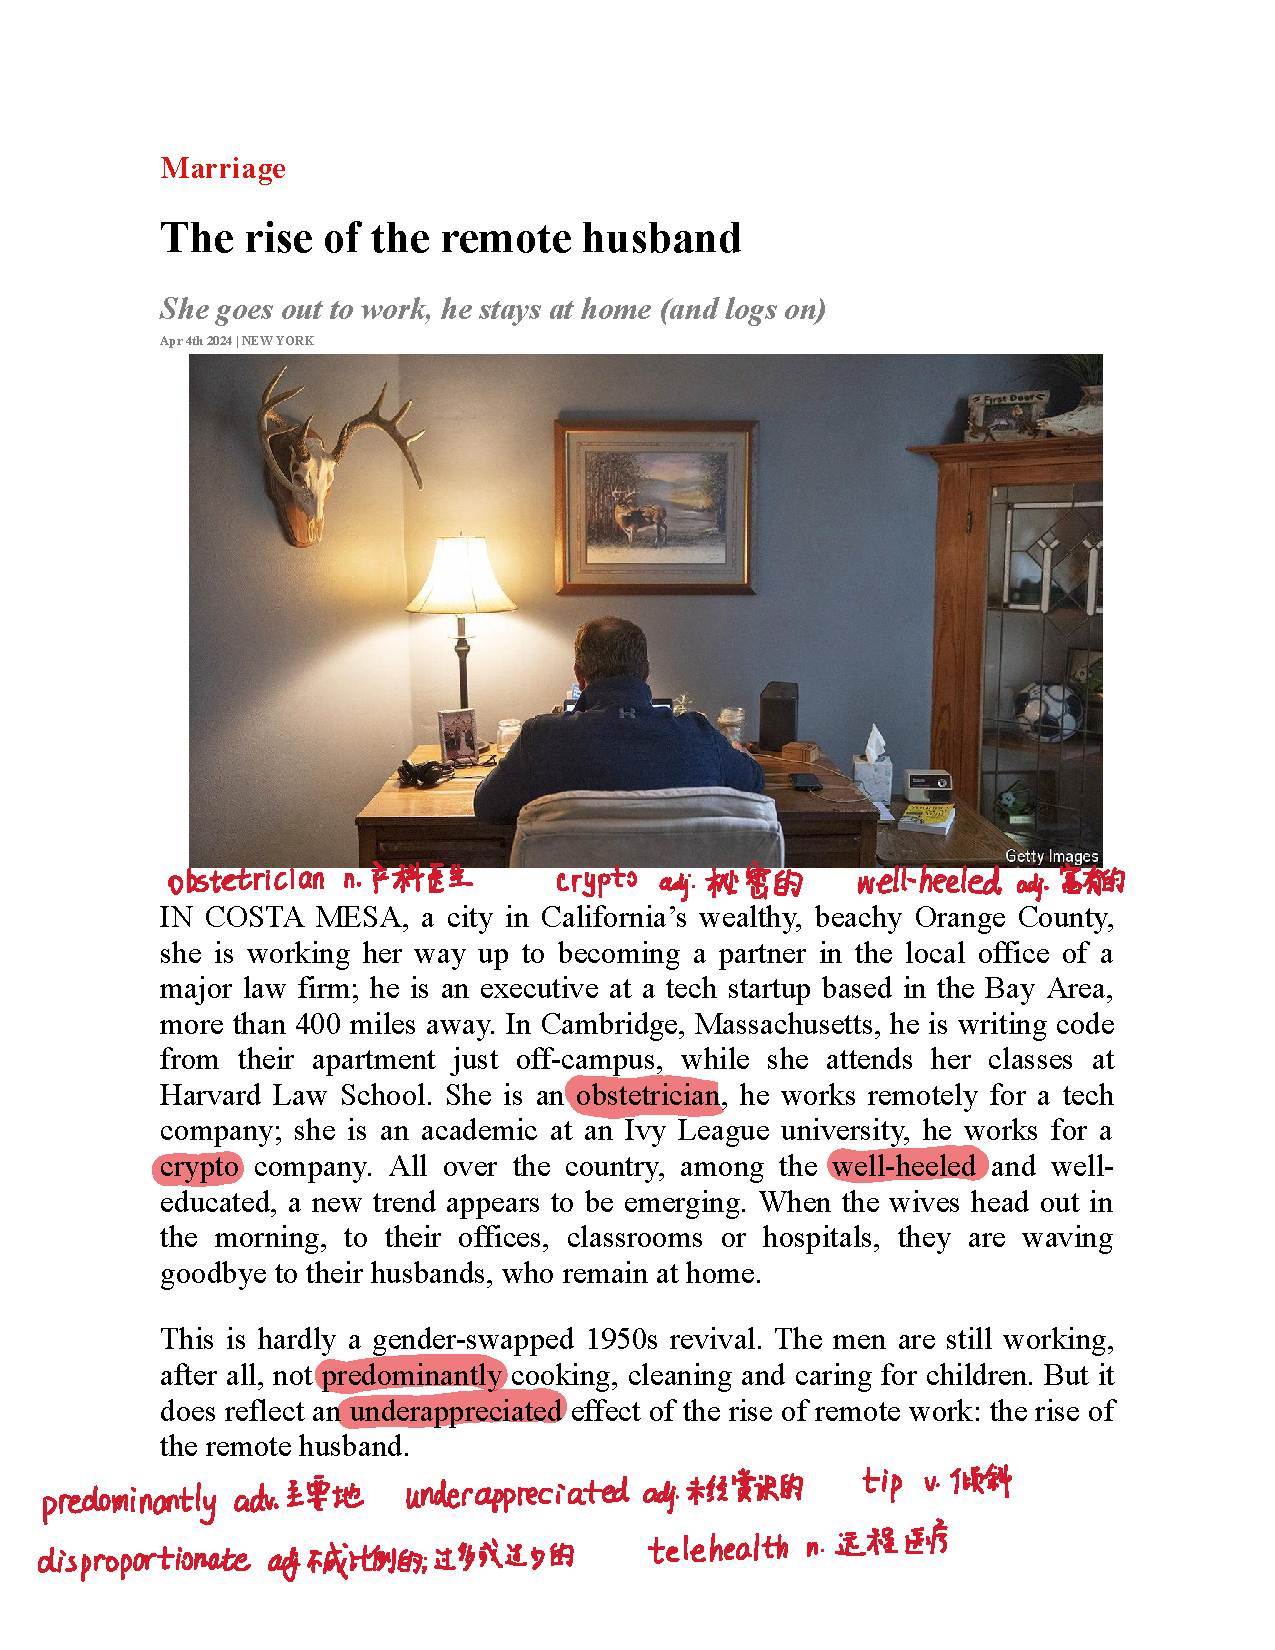
\includepdf[pages={1-3}]{第七周外刊.pdf}
\begin{itemize}
    \item [1.]Ivy League 常春藤名校联盟
    \begin{multicols}{2}
        \begin{itemize}
            \item [a.]哈佛Harvard
            \item [b.]宾大University of Pennsylvania
            \item [c.]耶鲁Yale University
            \item [d.]普林斯顿Princeton University
            \item [e.]哥大Columbia University
            \item [f.]布朗Brown University
            \item [g.]康奈尔Cornell University
            \item [h.]达特茅斯Dartmouth College
        \end{itemize}
    \end{multicols}
    
    \item [2.]crypto company 加密公司
    \item [3.]underappreciated adj. 尚未被重视的,低估的


    e.g.\qquad Yet, \textbf{an underappreciated effect of} increased 
    social media usage \textbf{is its impact on }
    interpersonal skills. \textbf{While much focus is 
    placed on the benefits of }instant communication, 
    \textbf{such as }increased information sharing and 
    connectivity, \textbf{the consequences of }
    reduced face-to-face interactions on our 
    ability to effectively communicate and 
    empathize with others \textbf{are often overlooked. 
    This decline in }social skills can lead to 
    a deeper sense of isolation and misunderstanding 
    in society, \textbf{despite }the virtual connectivity.

    (...的坏处常常被低估,它的可能后果是...)
    \item [4.]swap v. 互换、交换
        
    swap A for B 把A换成B(可用于作文中措施段,用...替换...)


    congestion n. 交通堵塞


    e.g.\qquad ...(环保措施), which will encourage people to swap car travel 
    for cycling or walking to reduce traffic congestion 
    and air pollution.
    \item [5.]predominantly adv. 主要
    
    bolster v. 增强
    
    e.g.\qquad While traditional teaching methods and digital 
    tools play crucial roles in education, it is 
    predominantly online resources and software 
    applications that are shaping the way students 
    learn in many cultures. This trend towards 
    digitalization in education reflects broader societal 
    shifts towards technology reliance.
    \item [6.]disproportionate adj. 不匀称的,不均衡的
    
    a large proportion of ... ...的很大一部分

    a sense of proportion 有轻重缓急之分,分寸感

    out of proportion 比例失调,不匀称
    \item [7.]tip v. 倾斜,变化
    
    the scales are tipping as ... 随着...,情况正在反转

    e.g.1\qquad While artificial intelligence was once the domain 
    of science fiction, \textbf{the scales are tipping as }
    AI becomes an integral part of daily life, from 
    smart home devices to personalized healthcare solutions.

    underscore v. 强调
    
    traction n. 拉力

    gain traction 发展

    gig n. 临时工作

    e.g.2\qquad The conventional 9-to-5 office job has been the 
    standard for decades, symbolizing stability and 
    professional success. But \textbf{the scales are tipping, as }
    the gig economy and remote work \textbf{gain traction}. 
    This transformation underscores a reevaluation 
    of traditional work values, emphasizing 
    the importance of work-life balance, autonomy, 
    and \textbf{leveraging }technological advancements 
    to facilitate working from any location.

    the tip of the iceberg 冰山一角

    e.g.3\qquad These examples are just \textbf{the tip of the iceberg}, 
    but they demonstrate how helping 
    customers get more use of their materials can 
    transform value chains and operations.

    the tipping point 转折点

    e.g.4\qquad It looks like it---after all, 
    2012 was \textbf{the tipping point }when more than half 
    of Americans began owning smartphones.

    \item [8.]be tied to 被...束缚
    
    e.g.\qquad I dont't want to be tied to a steady job. 我不想被工作束缚
    $\rightarrow$我不想要一成不变的工作
    \item [9.]in aggregate 总的来说
    \item [10.]the short end of the stick 不利地位
    \item [11.]myopic adj. 目光短浅的
    
    e.g.\qquad (先说一个荒谬的观点)But the 
    view is myopic.(再接下文)
    \item [12.]disadvantage v. 对...不利
    
    e.g.1\qquad This may appear another development 
    where remote work \textbf{disadvantages }workers 
    by blurring the lines between personal and 
    professional life. \textbf{But that view is 
    myopic.} In reality, remote work offers 
    unprecedented flexibility, empowering individuals 
    to design work schedules that harmonize with 
    their personal lives and responsibilities.

    e.g.2\qquad This may sound like another example 
    of how technological advancements lead to greater 
    social isolation. \textbf{But that view is myopic}. 
    In reality, technology has the power to connect 
    people across geographical boundaries like 
    never before, fostering new communities and enabling 
    closer relationships despite physical distance.

    testament n. 证据,证明

    nuanced adj. 微妙的,细致入微的

    e.g.3\qquad This may sound like another testament
    to the belief that tecchnology can solve all our 
    problems. \textbf{But that view is myopic}. 
    In reality, while technological advancements 
    have undoubtedly improved many aspects of our 
    lives, they also pose new ethical dilemmas and 
    challenges. Issues such as privacy invasion, 
    data security, and the digital divide require a 
    nuanced understanding of ethics beyond mere 
    technical solutions.
\end{itemize}

\chapter{长难句}
\section{Week7}
\begin{multicols}{2}
    \begin{itemize}
        \item [1.]watershed n. 分水岭,转折点
        \item [2.]manifest v. 显示,表明
        \item [3.]postgraduate n. 研究生
        \item [4.]scholar n. 学者,奖学金获得者
    \end{itemize}
\end{multicols}

\chapter{CS61B}
\section{Section 1}
\begin{multicols}{2}
    \begin{itemize}
        \item [1.]verbose adj. 冗长啰嗦的
        \item [2.]syntax n. 语法
        \item [3.]syntactic adj. 语法的
        \item [4.]denote v. 标志
        \item [5.]semicolon n. 分号
        \item [6.]compiler n. 编译器
        \item [7.]interpreter n. 解释程序
        \item [8.]bytecode n. 字节码
        \item [9.]loop n. 循环
    \end{itemize}
\end{multicols}



\end{document}